%!TEX TS-program = xelatex
%!TEX encoding = UTF-8 Unicode
\documentclass{article}
\usepackage[provide=*,dutch]{babel}

\usepackage{geometry}
\geometry{a4paper}
\usepackage[utf8]{inputenc}
\usepackage{enumitem}
\usepackage{hyperref}
\usepackage{graphicx}
\usepackage{tcolorbox}
\usepackage{float}
\usepackage{tabularx}
\hyphenation{wacht-tijd}
\hyphenation{wacht-tijden}
\setlength{\textheight}{240truemm}
% For better header handling
\usepackage{fancyhdr}
\pagestyle{fancy}
\fancyhf{}
\lhead{Ontwerpdocument Ingensche Veer}
\chead{IPASS}
\rhead{Vincent van Setten - 1734729}
\rfoot{Pagina \thepage}

% For colored text
\usepackage{xcolor}

\title{IPASS Plan van Aanpak}
\author{Vincent van Setten}

\begin{document}

\begin{titlepage}
    \begin{center}
        \vspace*{.6cm}
        \Huge
        \textbf{Ontwerpdocument }\\
        \vspace{0.2cm}
        \LARGE 
        \textbf{Ingensche Veer} \\
  
        \normalsize
  
  
        \vspace{1cm}
        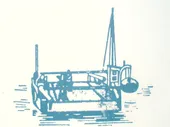
\includegraphics[width=0.7\textwidth]{images/iv.png}
        \vspace{1cm}
        \Large\\
        \textbf{In opdracht van}\\
        \large
        \textbf{University of Applied Sciences Utrecht} \\
        
\includegraphics[width=0.2\textwidth]{images/logouni.jpg}
  
        \vfill
      \end{center}
      \textbf{Datum:} \today \\
      \textbf{Versie:} 2.0 \\
      \textbf{Auteur:} Vincent van Setten \\
      \textbf{Studentnummer:} 1734729 \\
      \textbf{Klas:} V1C\\
  
  \end{titlepage}
  
  % ToC
  \tableofcontents
  \pagebreak 

  \section{Revisie Historie}
  \begin{table}[h]
      \centering
      \begin{tabular}{|c|c|c|p{5cm}|}
          \hline
          \textbf{Versie} & \textbf{Datum} & \textbf{Omschrijving}  \\
          \hline
          1.0  & 04-06-2024 & Eerste Versie \\
          2.0 & 30-06-2024 & Tweede Versie \\
          \hline
  
      \end{tabular}
      \caption{Versiegeschiedenis}
  \end{table}
  \pagebreak

\section{Inleiding}
Tussen Ingen en Elst (Utrecht) ligt een veerpont. Deze gaat eigenlijk constant op en neer, zonder een vast tijdschema.
De veerpont is vrij groot en is voor zowel voetgangers, als auto's en fietsen. Er passen ongeveer 20 auto's op en een groot aantal fietsers en voetgangers.
De veerpont is relatief druk. Er worden dagelijks honderden mensen overgezet en is erg belangrijk voor de inwoners rondom Ingen en Elst. Het lastige met de drukte op de veerpont is dat het vaak in vlagen komt. De ene overtocht heeft slechts twee auto's en bij de volgende staan er zoveel dat niet alle auto's tegelijk over kunnen. Dit komt vooral omdat mensen niet weten wanneer de veerpont aankomt, waardoor veel mensen hem vaak net missen en vervolgens lang moeten wachten.
\par\smallskip 
Dat zorgt voor veel frustratie bij de klanten en veroorzaakt ook stress bij de schipper.
De kern van het probleem is dat klanten de aankomsttijd van de veerpont niet kunnen inschatten.
Een mogelijke oplossing voor dit probleem is de ontwikkeling van een webapplicatie die de huidige locatie van de veerpont weergeeft. Met deze applicatie kunnen klanten inschatten wanneer de veerpont aankomt, wat helpt bij het spreiden van de drukte en het verminderen van de wachttijden. Dit systeem zal gebruik maken van AIS-data om real-time informatie over de veerpont te bieden.
\par\smallskip 
De webapplicatie helpt ook met een ander probleem. Als het erg druk is, kan de baas van de veerpont extra hulp inschakelen. Momenteel gaat dat door puur te kijken op een bepaald moment hoe druk het is. 
Hiermee komt de hulp vaak net te laat, waardoor er een grote ophoping aan drukte ontstaat. Het is de bedoeling dat met de webapplicatie de schipper per overtocht kan aangeven hoe druk het is. Hiermee kan de baas zien wanneer er hulp nodig is, maar kan hiermee ook inschatten hoe druk het gaat worden op basis van historische data. 
\par\smallskip 
In dit ontwerpdocument wordt beschreven welke dingen er worden opgeleverd aan het eind van het IPASS project, hoe het project wordt aangepakt en er uiteindelijk uit gaat zien.
Ook worden de risico's en de planning van het project beschreven.


\section{Overzicht van het systeem}


\section{Use Cases}
\begin{figure}[H]
    \centering
    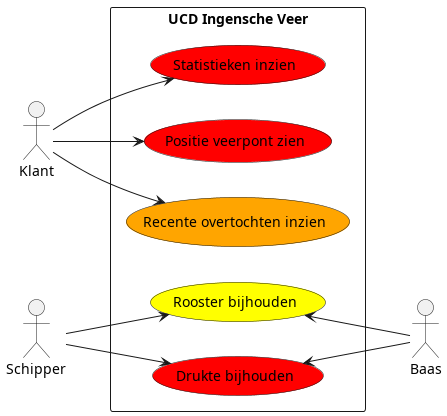
\includegraphics[width=0.7\textwidth]{images/ucd.png}
    \caption{Use Case Diagram - Ingensche Veer}
    \label{fig:ucd}
\end{figure}

In het use case diagram in figuur \ref{fig:ucd} zie je de verschillende use cases. Deze zijn gekleurd naar het MoSCoW model. Rode use cases zijn Must haves, oranje use cases zijn Should haves, gele use cases zijn Could haves en groene use cases zijn Won't haves.
Het use case diagram laat alleen de daadwerkelijke geimplementeerde use cases zien. 
Terugblikkend op het Plan van Aanpak is er vrij veel geimplementeerd.
Van de Must Haves is alles geimplementeerd. van de Should Haves is ook alles geimplementeerd. Van de Could Haves zijn de roosters geimplementeerd, maar de geschatte drukte, snelheid van invididuele schippers en integratie met weersomstandigheden niet. Van de Won't Haves is niks geimplementeerd.
Alle statistieken van de Must haves, could haves and should haves zijn geimplementeerd onder de enkele use case 'statistieken inzien'.


\subsection{Actoren}

\begin{table}[H]
    \centering
    \begin{tabularx}{\textwidth}{|l|X|}
        \hline
        \textbf{Actoren} & \textbf{Omschrijving}  \\
        \hline
        Baas & De baas is de eigenaar van de veerpont. \\
        \hline
        Klant  & De klant is de persoon die gebruik maakt van de veerpont. \\
        \hline
        Schipper & De schipper is de persoon die de veerpont vaart. \\
        \hline

    \end{tabularx}
    \caption{Actoren}
\end{table}

\subsection{Use case beschrijvingen en wireframes}
\subsubsection{UC01 - Bekijk locatie veerpont}
\begin{table}[H]
    \centering
    \begin{tabularx}{\textwidth}{|l|X|}
        \hline
        \textbf{ID:} UC01 & \textbf{Use Case Naam:} Bekijk locatie veerpont  \\
        \hline
        \textbf{Actoren:} & Klant \\
        \hline
        \textbf{Samenvatting:}  & De klant kan de actuele positie van de veerpont inzien op een kaart \\
        \hline 
        \textbf{Precondities:} & De veerpont stuurt AIS signalen en deze worden via de API ontvangen. \\
        \hline
        \textbf{Scenario:} & \begin{enumerate}
            \item De klant opent de webapplicatie
            \item Systeem haalt de actuele locatie van de veerpont op.
            \item Systeem toont de locatie van de veerpont op een kaart.
            \item De klant kan de locatie van de veerpont inzien.
        \end{enumerate} \\
        \hline 
        \textbf{Postcondities:} & nvt \\ 
        \hline

    \end{tabularx}
    \caption{Use Case Beschrijving UC01 - Bekijk locatie veerpont}
\end{table}

\begin{figure}[H]
    \centering
    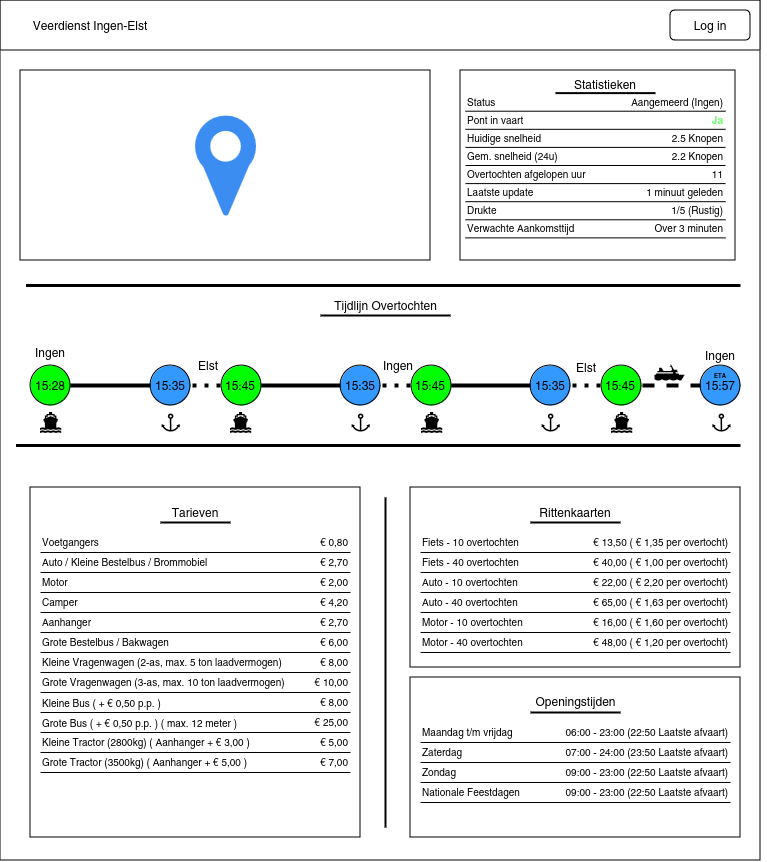
\includegraphics[width=0.8\textwidth]{images/wireframe_startpagina.png}
    \caption{Wireframe UC01 - Locatie veerpont bekijken}
    \label{fig:wf1}
\end{figure}

\section{Modellen}
\subsection{Domeinmodel}
\begin{figure}[H]
    \centering
    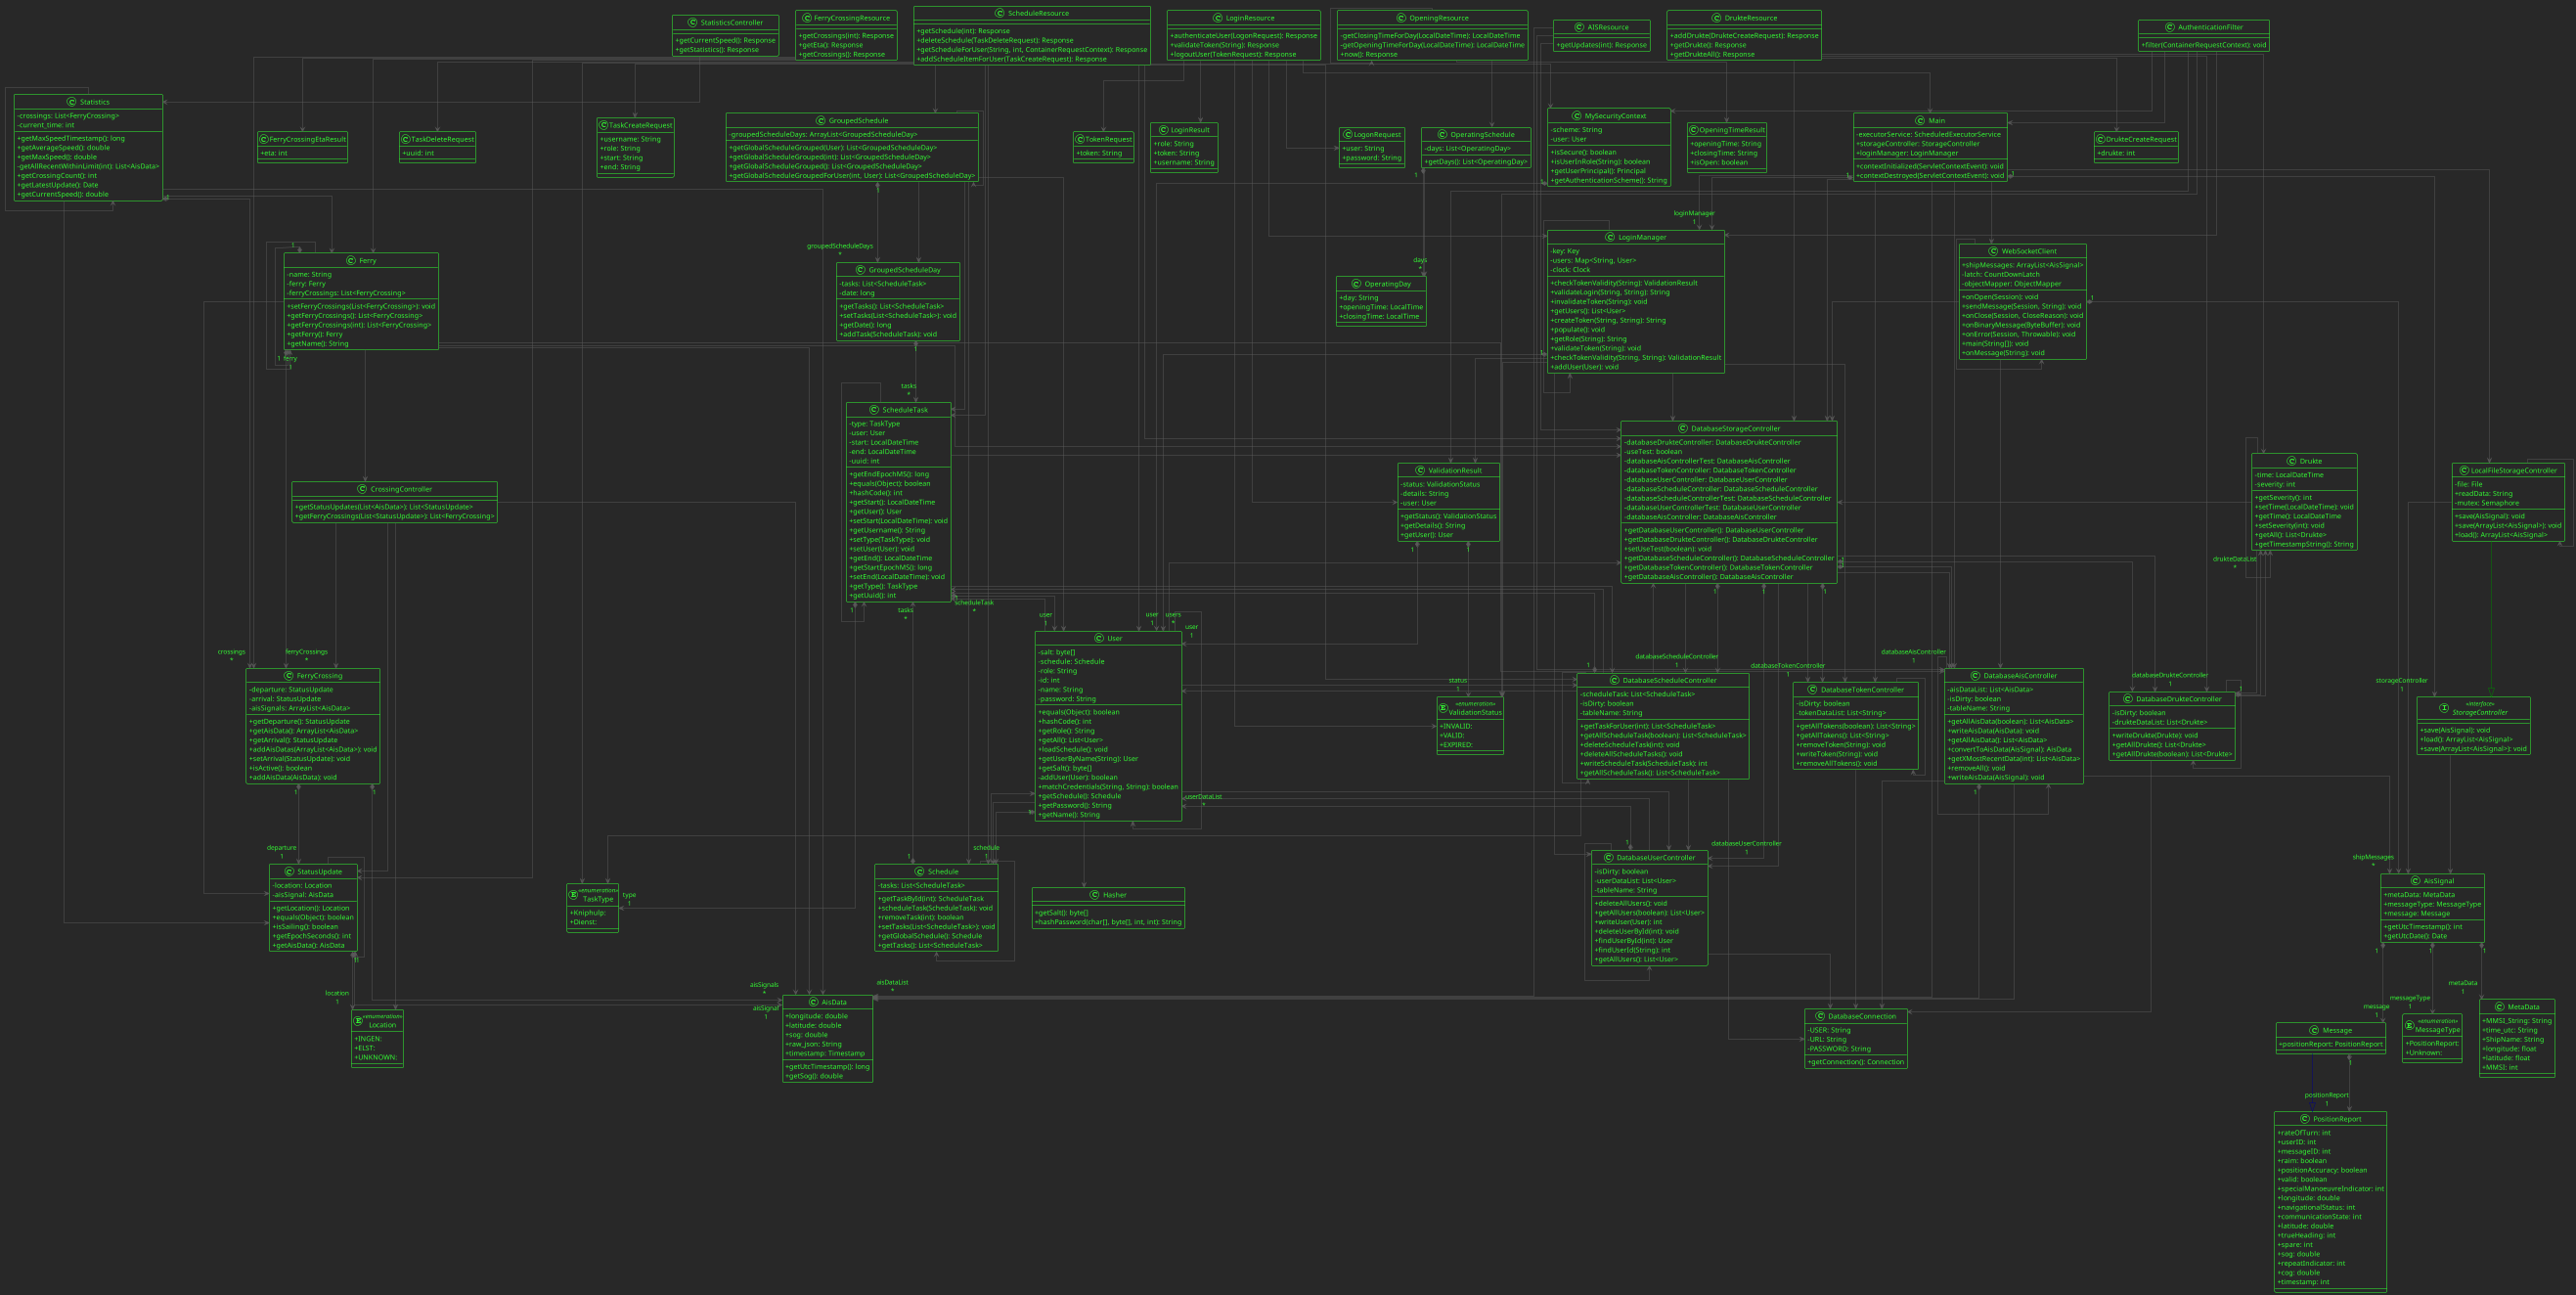
\includegraphics[width=1\textwidth]{images/FunctioneelKlassendiagram.png}
    \caption{Functioneel Domeinmodel - Ingensche Veer}
    \label{fig:dm}
\end{figure}
In het domeinmodel in figuur \ref{fig:dm} zie je elke klassen in mijn implementatie. Bovenin zijn de verschillende resources te zien. De resource klassen regelen de API calls. Aan deze klassen zijn verschillende andere klassen gekoppeld die ze nodig hebben. Dit zijn veelal data klassen. Zo gebruiken de resources veel 'request' en 'result' klassen, zoals de TaskCreateRequest. Dit is een simpele klasse die helpt met het serialiseren en deserialiseren van de objecten naar de frontend. 
In het midden van het model zijn een aantal Database controller klassen. De klasse 'DatabaseStorageController' is de storage controller die weer verschillende DatabaseController klassen heeft. Deze klassen maken verbinding met hun eigen database tabel. Zo is DatabaseAisController verantwoordelijk voor de tabel met de AIS signalen in de database.
Rechtsonderin het diagram is de AisSignal klassen te zien, samen met de subklassen. Dit zijn simpelweg json implemtatie klassen, om de inkomende json data te kunnen parsen.
De testklassen zijn buiten beschouwing gelaten in dit diagram, omdat deze niet relevant zijn voor het domeinmodel en het diagram onnodig nog groter maken.


\subsection{Business Rules}
Bij het domeinmodel in  figuur \ref{fig:dm} horen de volgende business rules:
\begin{enumerate}
    \item \textbf{Attribute Rule:} Een veerpont heeft minimaal een schippers.
    \item \textbf{Attribute Rule:} Een schipper heeft altijd maar één baas.
    \item \textbf{Entity Rule:} Elk AisSignaal heeft een snelheid, positie en tijd.
    \item \textbf{Entity Rule:} Elke gebruiker heeft een gebruikersnaam en wachtwoord.
    \item \textbf{Tuple Rule:} De datum van het verteksignaal is altijd kleiner dan de datum van het aankomstsignaal.
\end{enumerate} 

\subsection{Datamodellen}
\begin{figure}[H]
    \centering
    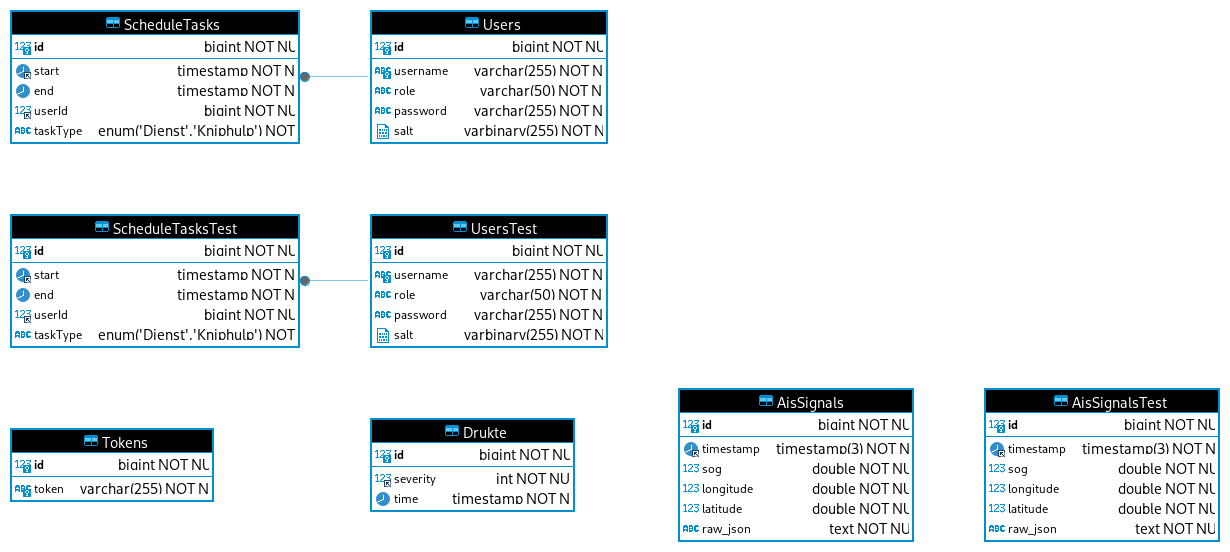
\includegraphics[width=1\textwidth]{images/erd.png}
    \caption{Database ERD - Ingensche Veer}
    \label{fig:erd}
\end{figure}
In figuur \ref{fig:erd} is het ERD van de database te zien. Sommige tabellen hebben een kopie. Deze heten <tabel>Test. Dit zijn tabellen die gebruikt worden tijdens de tests, zodat deze niet de echte data aantasten.
Ik zal de entiteiten hieronder kort toelichten.
\begin{enumerate}
    \item \textbf{ScheduleTasks}: Deze tabel bevat een taak. Een taak is een dienst op de veerpont. Deze is gekoppeld aan een gebruiker.
    \item \textbf{Users}: Deze tabel bevat de gebruikers en inlogdata van de gebruikers.
    \item \textbf{Tokens}: Deze tabel bevat de JWT tokens. Deze tabel is eigenlijk onnodig en dit had lokaal gedaan kunnen worden. Ik kwam er pas later achter dat tokens niet hoeven te persisten, omdat deze geinvalidate worden zodra de applicatie opnieuw opstart.
    \item \textbf{Drukte}: Deze tabel bevat een 'drukte' signaal. Een schipper kan deze doorgeven, wat de baas vervolgens weer kan inzien.
    \item \textbf{AisSignals}: Deze tabel bevat de AIS data. Dit zijn de signalen die de veerpont uitzendt.
\end{enumerate}
\textit{Ik heb geen fysiek of conceptueel datamodel gemaakt, omdat ik dit nooit heb gehad. Ik heb een oude versie van modelling gevolgd(in 2019) en dit niet gehad.}

\section{Technologieen}
\begin{enumerate}
    \item UML
    \item Java 
    \item HTML 
    \item CSS 
    \item Javascript 
    \item Jax-RS(Rest)
    \item HTTP-Protocol 
    \item MySQL
\end{enumerate}

\section{Overdracht} 
\subsection{Installatie}
\begin{enumerate}
    \item Clone de repository  
    \item Ga naar de frontend folder 
    \item Run 'npm install'
    \item Run 'npm run build'
    \item Ga terug naar de source folder 
    \item Open het project in intellij idea 
    \item Laad de maven dependencies in de pom.xml 
    \item Stel de applicatie in als tomcat applicatie
    \item Run de applicatie
\end{enumerate}
\subsection{Wachtwoorden}
\begin{itemize}
    \item \textbf{Vincent}: admin 
    \item \textbf{Stephan}: schipper 
    \item \textbf{Vincentvl}: schipper 
    \item \textbf{Baas}: baas
\end{itemize}


\section{Referenties}
Er zijn geen referenties.

\end{document}